\chapter{Diode Circuit II}


\section{Objectives}
\begin{itemize}
    \item To verify a half-wave diode rectifier circuit
    \item To verify clipper circuits and clamper circuits
\end{itemize}

\section{Materials}
\begin{itemize}
    \item Breadboard
    \item Capacitors
    \item DC power supply
    \item Digital Multi-Meter
    \item \hyperref[1N4148]{Diode (1N4148)}
    \item Function Generator
    \item Oscilloscope
    \item Resistors
\end{itemize}

\section{Introduction}
In this experiment, we are going to verify the half-wave diode rectifier circuit and clipper circuits and clamper circuits. Function Generator, DC sources, resistors, and diodes will be used to construct the circuits, the digital multi-meter and oscilloscope are used to measure and observe the data to find the relationship between them.\par
    \subsection{Circuits}
        \begin{itemize}
            \item \textbf{Half-wave Diode Rectifier}\par
            By using the diode's characteristic of allowing current to flow in only one direction, it allows the diode circuit converting alternating current (AC) to direct current (DC) by allowing only one half of the input AC signal to pass through.
            
            \item \textbf{Clipper and Clamper Circuits}\par
            \begin{table}[h]
            \centering
            \begin{tabular}{|p{3cm}|p{4cm}|p{4cm}|}
                \hline
                \textbf{Feature} & \textbf{Clipper Circuit} & \textbf{Clamper Circuit} \\
                \hline
                \textbf{Function} & Clips or limits the amplitude of the signal. & Shifts the DC level of the signal without clipping. \\
                \hline
                \textbf{Effect on Signal} & Reduces the signal's amplitude. & Shifts the signal's baseline up or down. \\
                \hline
                \textbf{Components Used} & Diode (in series or parallel with the load). & Diode and capacitor. \\
                \hline
                \textbf{Output} & Clipped waveform (portion of the waveform removed). & Entire waveform shifted up or down. \\
                \hline
                \textbf{Applications} & Signal limitation, protection, waveform shaping. & Biasing, level shifting, baseline restoration. \\
                \hline
                \end{tabular}
            \caption{Comparison of Clipper and Clamper Circuits}
            \end{table}
            \FloatBarrier
            
        \end{itemize}
    \subsection{Circuit Diagram}
    \begin{figure}[h]

        \begin{subfigure}[h]{0.47\textwidth}
        \begin{center}
            \includesvg[width=1\linewidth]{Lab02/Lab2a.drawio.svg}
            \caption{A half-wave diode rectifier}
            \label{Lab2a}
        \end{center} 
        \end{subfigure}
    \hfill
    \vspace{0.2 cm}
        \begin{subfigure}[h]{0.47\textwidth}
        \begin{center}
            \includesvg[width=1\linewidth]{Lab02/Lab2b.drawio.svg}
            \caption{A clipper circuit with up limit}
            \label{Lab2b}
        \end{center}
        \end{subfigure}
    \vfill
    \vspace{0.2 cm}
        \begin{subfigure}[h]{0.47\textwidth}
        \begin{center}
            \includesvg[width=1\linewidth]{Lab02/Lab2c.drawio.svg} 
            \caption{A clipper circuit with two limits}
            \label{Lab2c}
        \end{center}
        \end{subfigure}
    \hfill
        \begin{subfigure}[h]{0.47\textwidth}
        \begin{center}
            \includesvg[width=1\linewidth]{Lab02/Lab2d.drawio.svg}
            \caption{A clamper circuit}
            \label{Lab2d}
        \end{center}
        \end{subfigure}
    \caption{Diode Circuits}
    \label{SDC}

    \end{figure}
\FloatBarrier
The R shown in the circuits represents 1k$\Omega$. And $R_1$ = 1k$\Omega$, $R_2$ = 10k$\Omega$.



\section{Detailed Procedures}
    \subsection{Analyzation}
    First, we analyze the relationship inside of each circuit.\par
    \begin{itemize}
        \item In figure. \ref{Lab2a}:\par
        \begin{equation}
            \begin{cases}
                V_o = V_s - V_\gamma & V_s \ge V_\gamma,~\text{D is on}\\
                V_o = 0 & V_s < V_\gamma,~\text{D is off}\\
            \end{cases}
        \label{l2eq1}
        \end{equation}
        
        \item In figure. \ref{Lab2b}:
        \begin{equation}
            \begin{cases}
                V_o = V_\gamma + V_s & V_B - V_\gamma \ge V_s,~\text{D is on}\\
                V_o = V_B & V_s > V_B - V_\gamma,~\text{D is off}\\
            \end{cases}
        \label{l2eq2}
        \end{equation}
            
        \item In figure. \ref{Lab2c}:
        \begin{equation}
            \begin{cases}
                V_o = V_{B_2} & V_s > V_{B_2} - V_\gamma,~\text{Both diodes off}\\
                V_o = V_{B_2} - R_2(\frac{V_{B_2}-V_\gamma-V_s}{R_1+R_2}) & V_\gamma \le V_s \le V_{B_2} - V_\gamma,~\text{$D_1$ on only}\\
                V_o = V_\gamma & V_\gamma > V_s,~\text{Both diodes on}\\
            \end{cases}
        \label{l2eq3}
        \end{equation}
            
        \item In figure. \ref{Lab2d}:
        \begin{equation}
            \begin{cases}
                V_o = V_p(sin\omega t-1) & V_s \ge 0,~\text{Diode on}\\
                V_o = V_s - V_C & V_s < 0,~\text{Diode off}\\
            \end{cases}
        \label{l2eq4}
        \end{equation}
    \end{itemize}
    \FloatBarrier

    \subsection{Procedures}
    We used digital multi-meter to measure data from the circuit. Estimate build-in voltage is 0.6V.
    \begin{itemize}
        \item For Fig.\ref{Lab2a},\par
            \begin{table}[h]
            \centering
            \begin{tabular}{|c|c|c|c|c|c|c|c|c|}
                \hline
                Vs   & -3     & -2.8   & -2.6   & -2.4   & -2.2   & -2    & -1.8  & -1.6   \\ \hline
                Vo   & 0      & 0      & 0      & 0      & 0      & 0     & 0     & 0      \\ \hline
                Theo & 0      & 0      & 0      & 0      & 0      & 0     & 0     & 0      \\ \hline
                Vs   & -1.4   & -1.2   & -1     & -0.8   & -0.6   & -0.4  & -0.2  & 0      \\ \hline
                Vo   & 0      & 0      & 0      & 0      & 0      & 0     & 0     & 0      \\ \hline
                Theo & 0      & 0      & 0      & 0      & 0      & 0     & 0     & 0      \\ \hline
                Vs   & 0.2    & 0.4    & 0.6    & 0.8    & 1      & 1.2   & 1.4   & 1.6    \\ \hline
                Vo   & 0.2m   & 10.48m & 101.3m & 0.2587 & 0.431  & 0.614 & 7993  & 0.9886 \\ \hline
                Theo & 0      & 0      & 0      & 0.2    & 0.4    & 0.6   & 0.8   & 1      \\ \hline
                Vs   & 1.8    & 2      & 2.2    & 2.4    & 2.6    & 2.8   & 3     &        \\ \hline
                Vo   & 1.1758 & 1.3674 & 1.561  & 1.752  & 1.9457 & 2.145 & 2.343 &        \\ \hline
                Theo & 1.2    & 1.4    & 1.6    & 1.8    & 2      & 2.2   & 2.4   &        \\ \hline
            \end{tabular}
            \end{table}
            \FloatBarrier
            \begin{figure}[h]
                \centering
                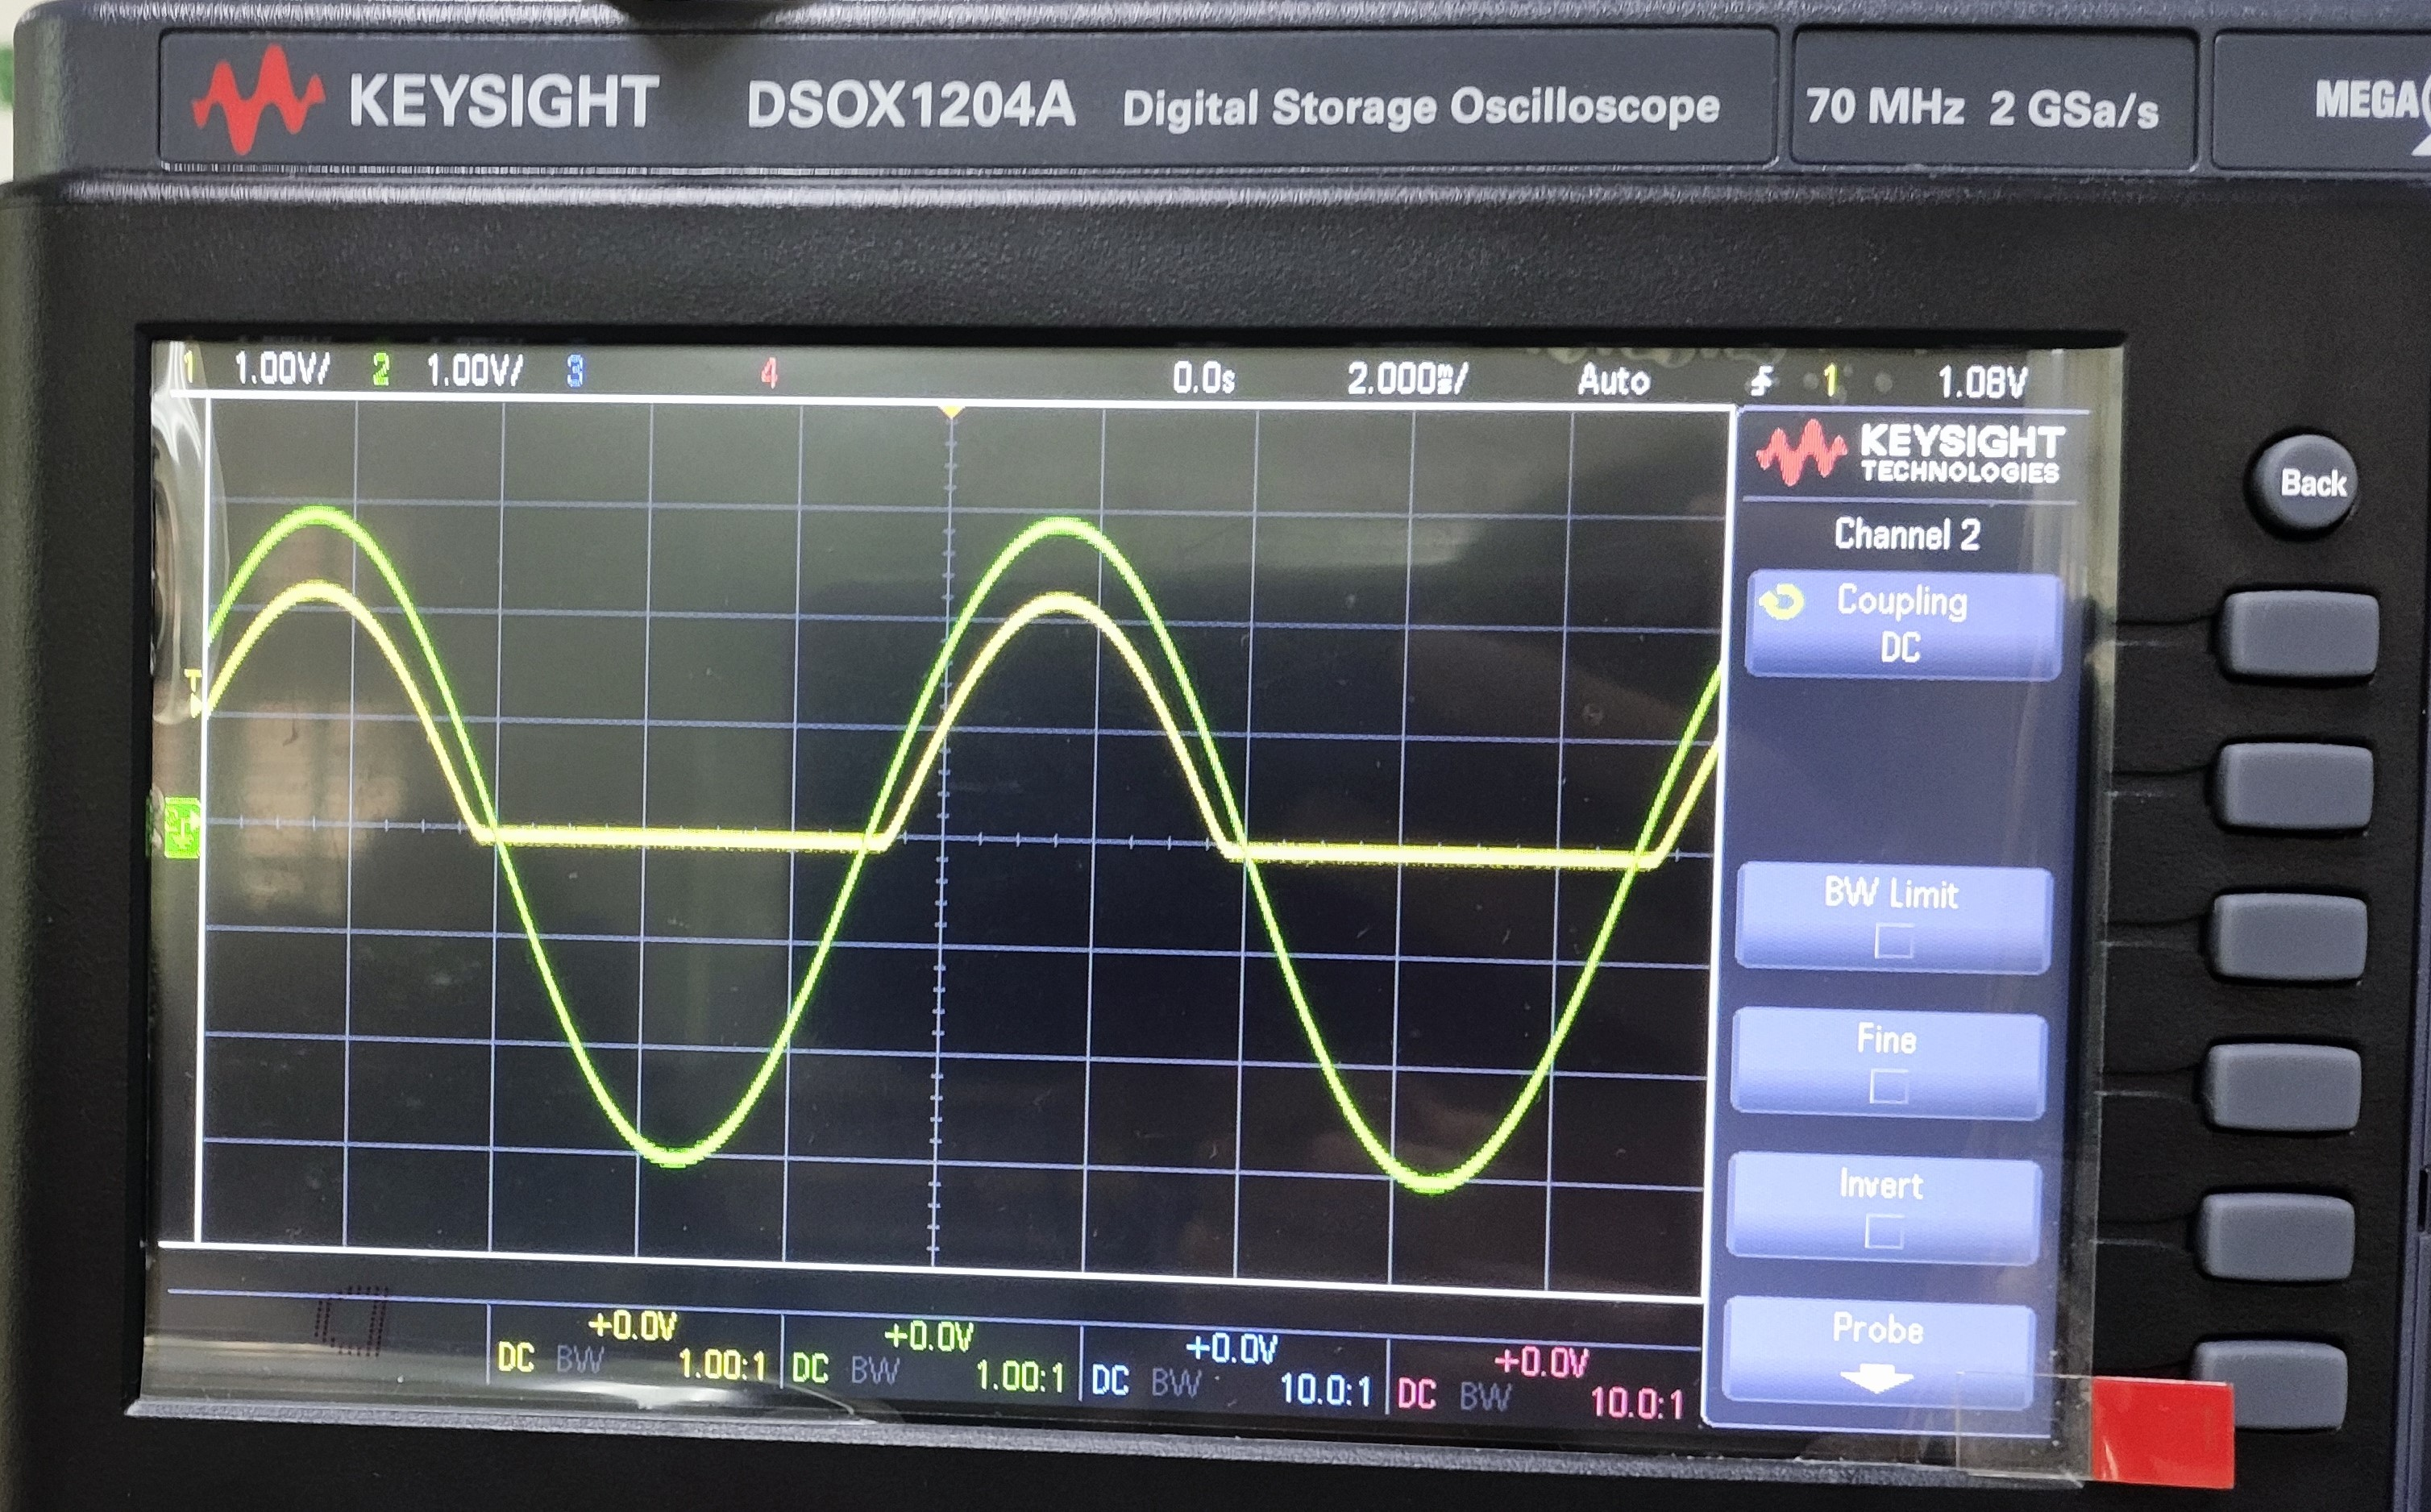
\includegraphics[width=0.65\linewidth]{Lab02/2.4_sin_halfWave.jpg}
                \caption{Sinusoidal Signal}
                \label{2.4sin}
            \end{figure}
            \FloatBarrier
            \begin{figure}[h]
                \centering
                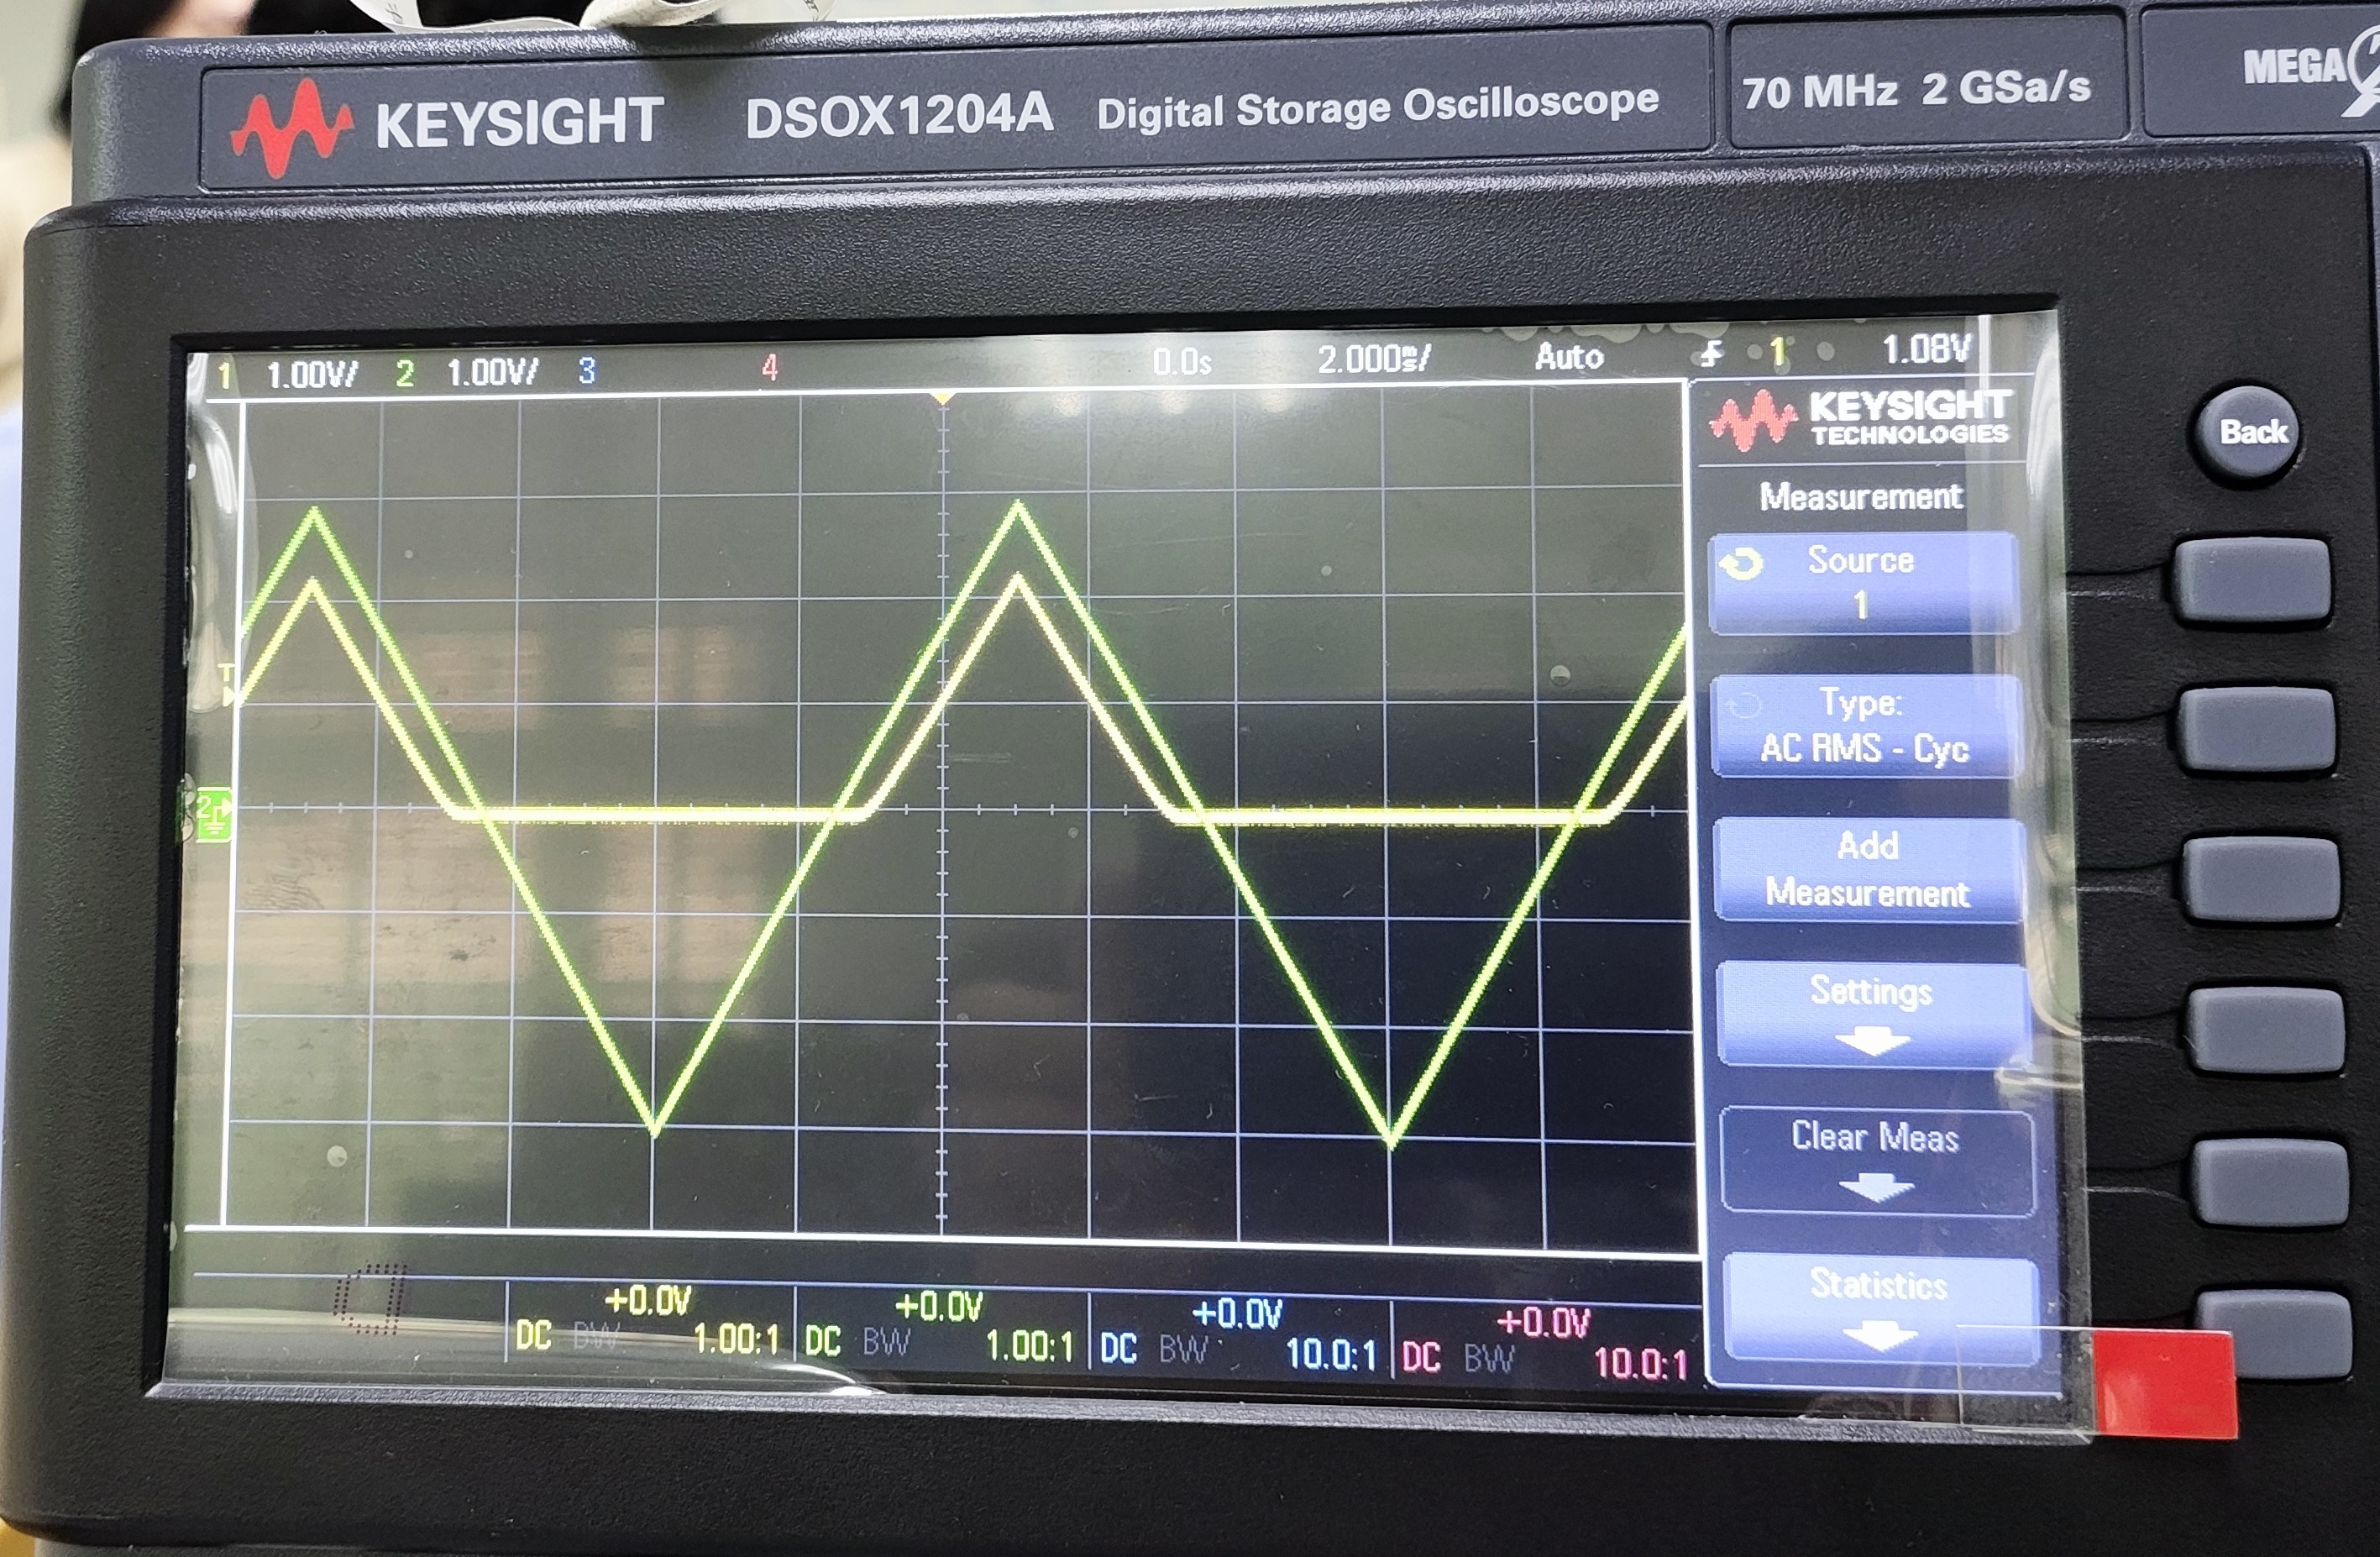
\includegraphics[width=0.65\linewidth]{Lab02/2.4_tri_halfWave.jpg}
                \caption{Triangular Signal}
                \label{2.4tri}
            \end{figure}
            \FloatBarrier
            From the Fig.\ref{2.4sin} and Fig.\ref{2.4tri}, we can tell that the output signal $V_o$ (Channel 1/Yellow) is lower than input signal $V_s$ (Channel 2/Green), and the negative axis of the output signal turns to zero. Former is because some of voltage is distributed to the diode, latter is because the negative axis signal is blocked by the diode. The latency of signal rising because the input signal need to dissipate voltage on diode, once input signal reaches threshold voltage it will start rising.
        \item For Fig.\ref{Lab2b},\par
            \begin{table}[h]
            \centering
            \begin{tabular}{|c|c|c|c|c|c|c|c|c|}
                \hline
                Vs   & -3     & -2.8   & -2.6   & -2.4   & -2.2  & -2     & -1.8   & -1.6   \\ \hline
                Vo   & -2.317 & -2.125 & -1.923 & -1.73  & -1.53 & -1.338 & -1.142 & -0.947 \\ \hline
                Theo & -2.4   & -2.2   & -2     & -1.8   & -1.6  & -1.4   & -1.2   & -1     \\ \hline
                Vs   & -1.4   & -1.2   & -1     & -0.8   & -0.6  & -0.4   & -0.2   & 0      \\ \hline
                Vo   & -0.754 & -0.564 & -0.364 & -0.177 & 0.015 & 0.208  & 0.388  & 0.568  \\ \hline
                Theo & -0.8   & -0.6   & -0.4   & -0.2   & 0     & 0.2    & 0.4    & 0.6    \\ \hline
                Vs   & 0.2    & 0.4    & 0.6    & 0.8    & 1     & 1.2    & 1.4    & 1.6    \\ \hline
                Vo   & 0.744  & 0.899  & 0.989  & 0.999  & 0.999 & 0.999  & 0.999  & 0.999  \\ \hline
                Theo & 0.8    & 1      & 1      & 1      & 1     & 1      & 1      & 1      \\ \hline
                Vs   & 1.8    & 2      & 2.2    & 2.4    & 2.6   & 2.8    & 3      &        \\ \hline
                Vo   & 0.999  & 0.999  & 0.999  & 0.999  & 0.999 & 0.999  & 0.999  &        \\ \hline
                Theo & 1      & 1      & 1      & 1      & 1     & 1      & 1      &        \\ \hline
            \end{tabular}
            \end{table}
            \FloatBarrier
            \begin{figure}[h]
                \centering
                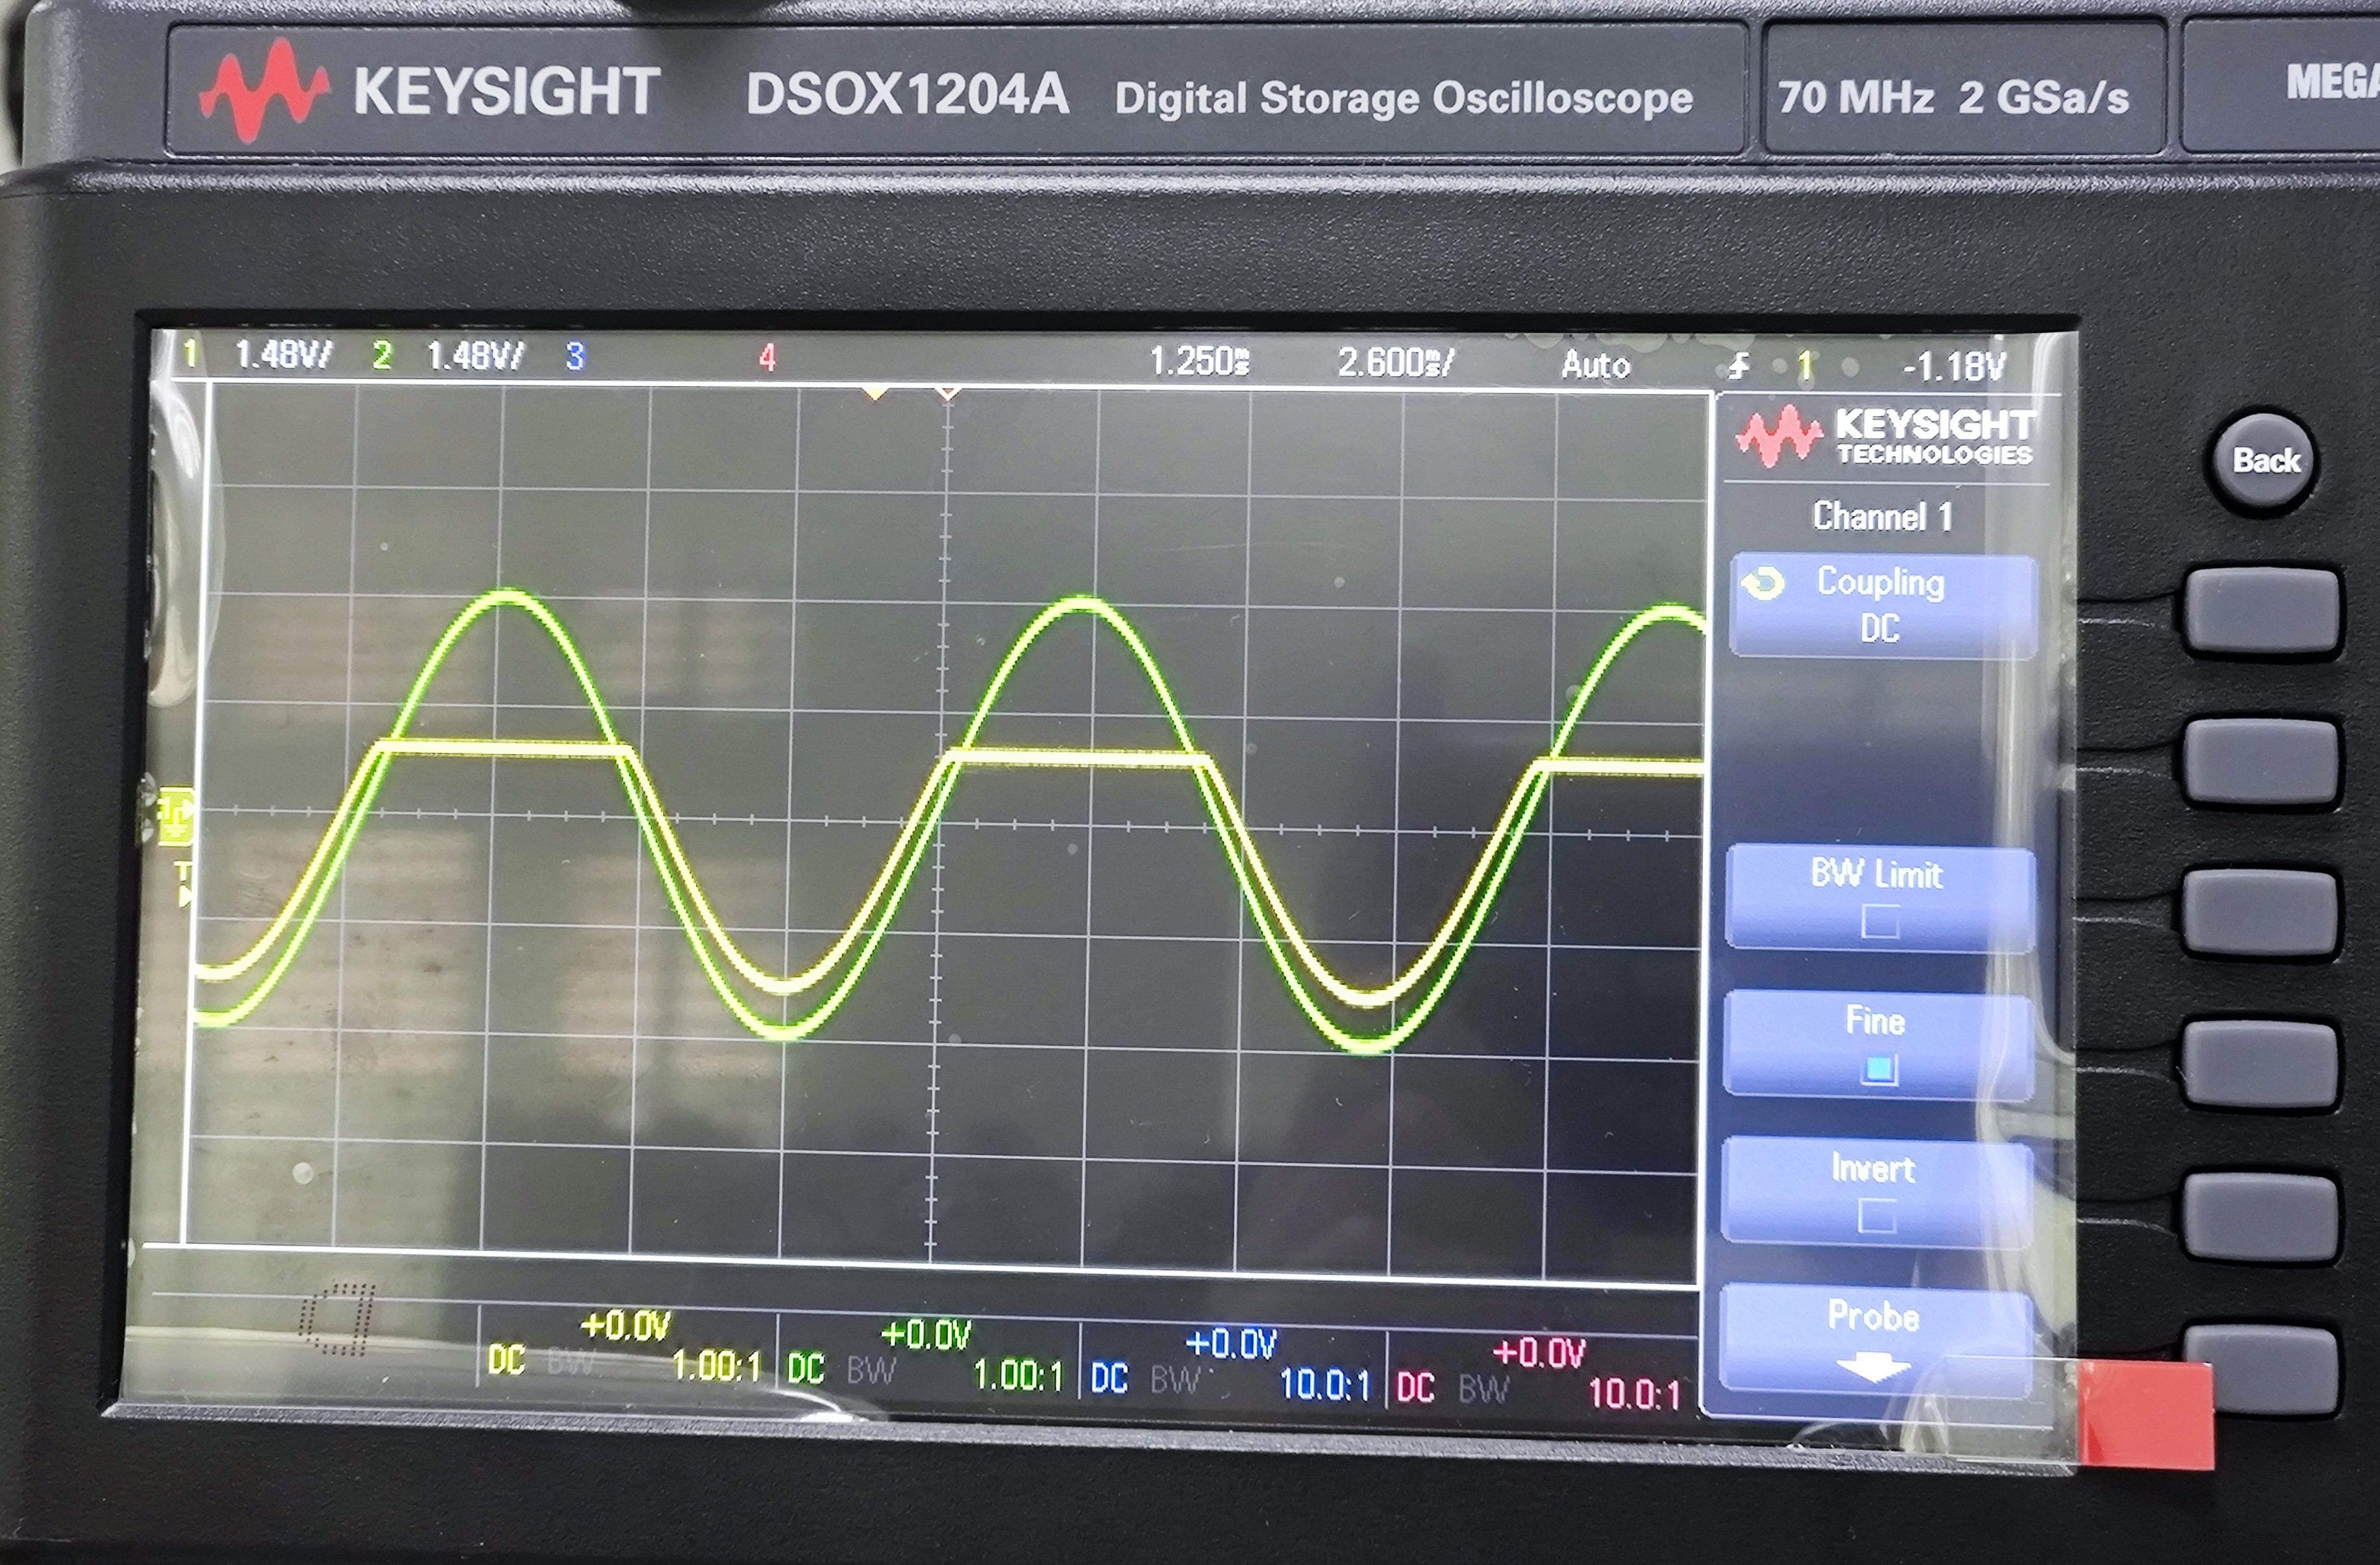
\includegraphics[width=0.65\linewidth]{Lab02/2.5_sin_clipper1.jpg}
                \caption{Sinusoidal Signal}
                \label{2.5sin}
            \end{figure}
            \FloatBarrier
            \begin{figure}[h]
                \centering
                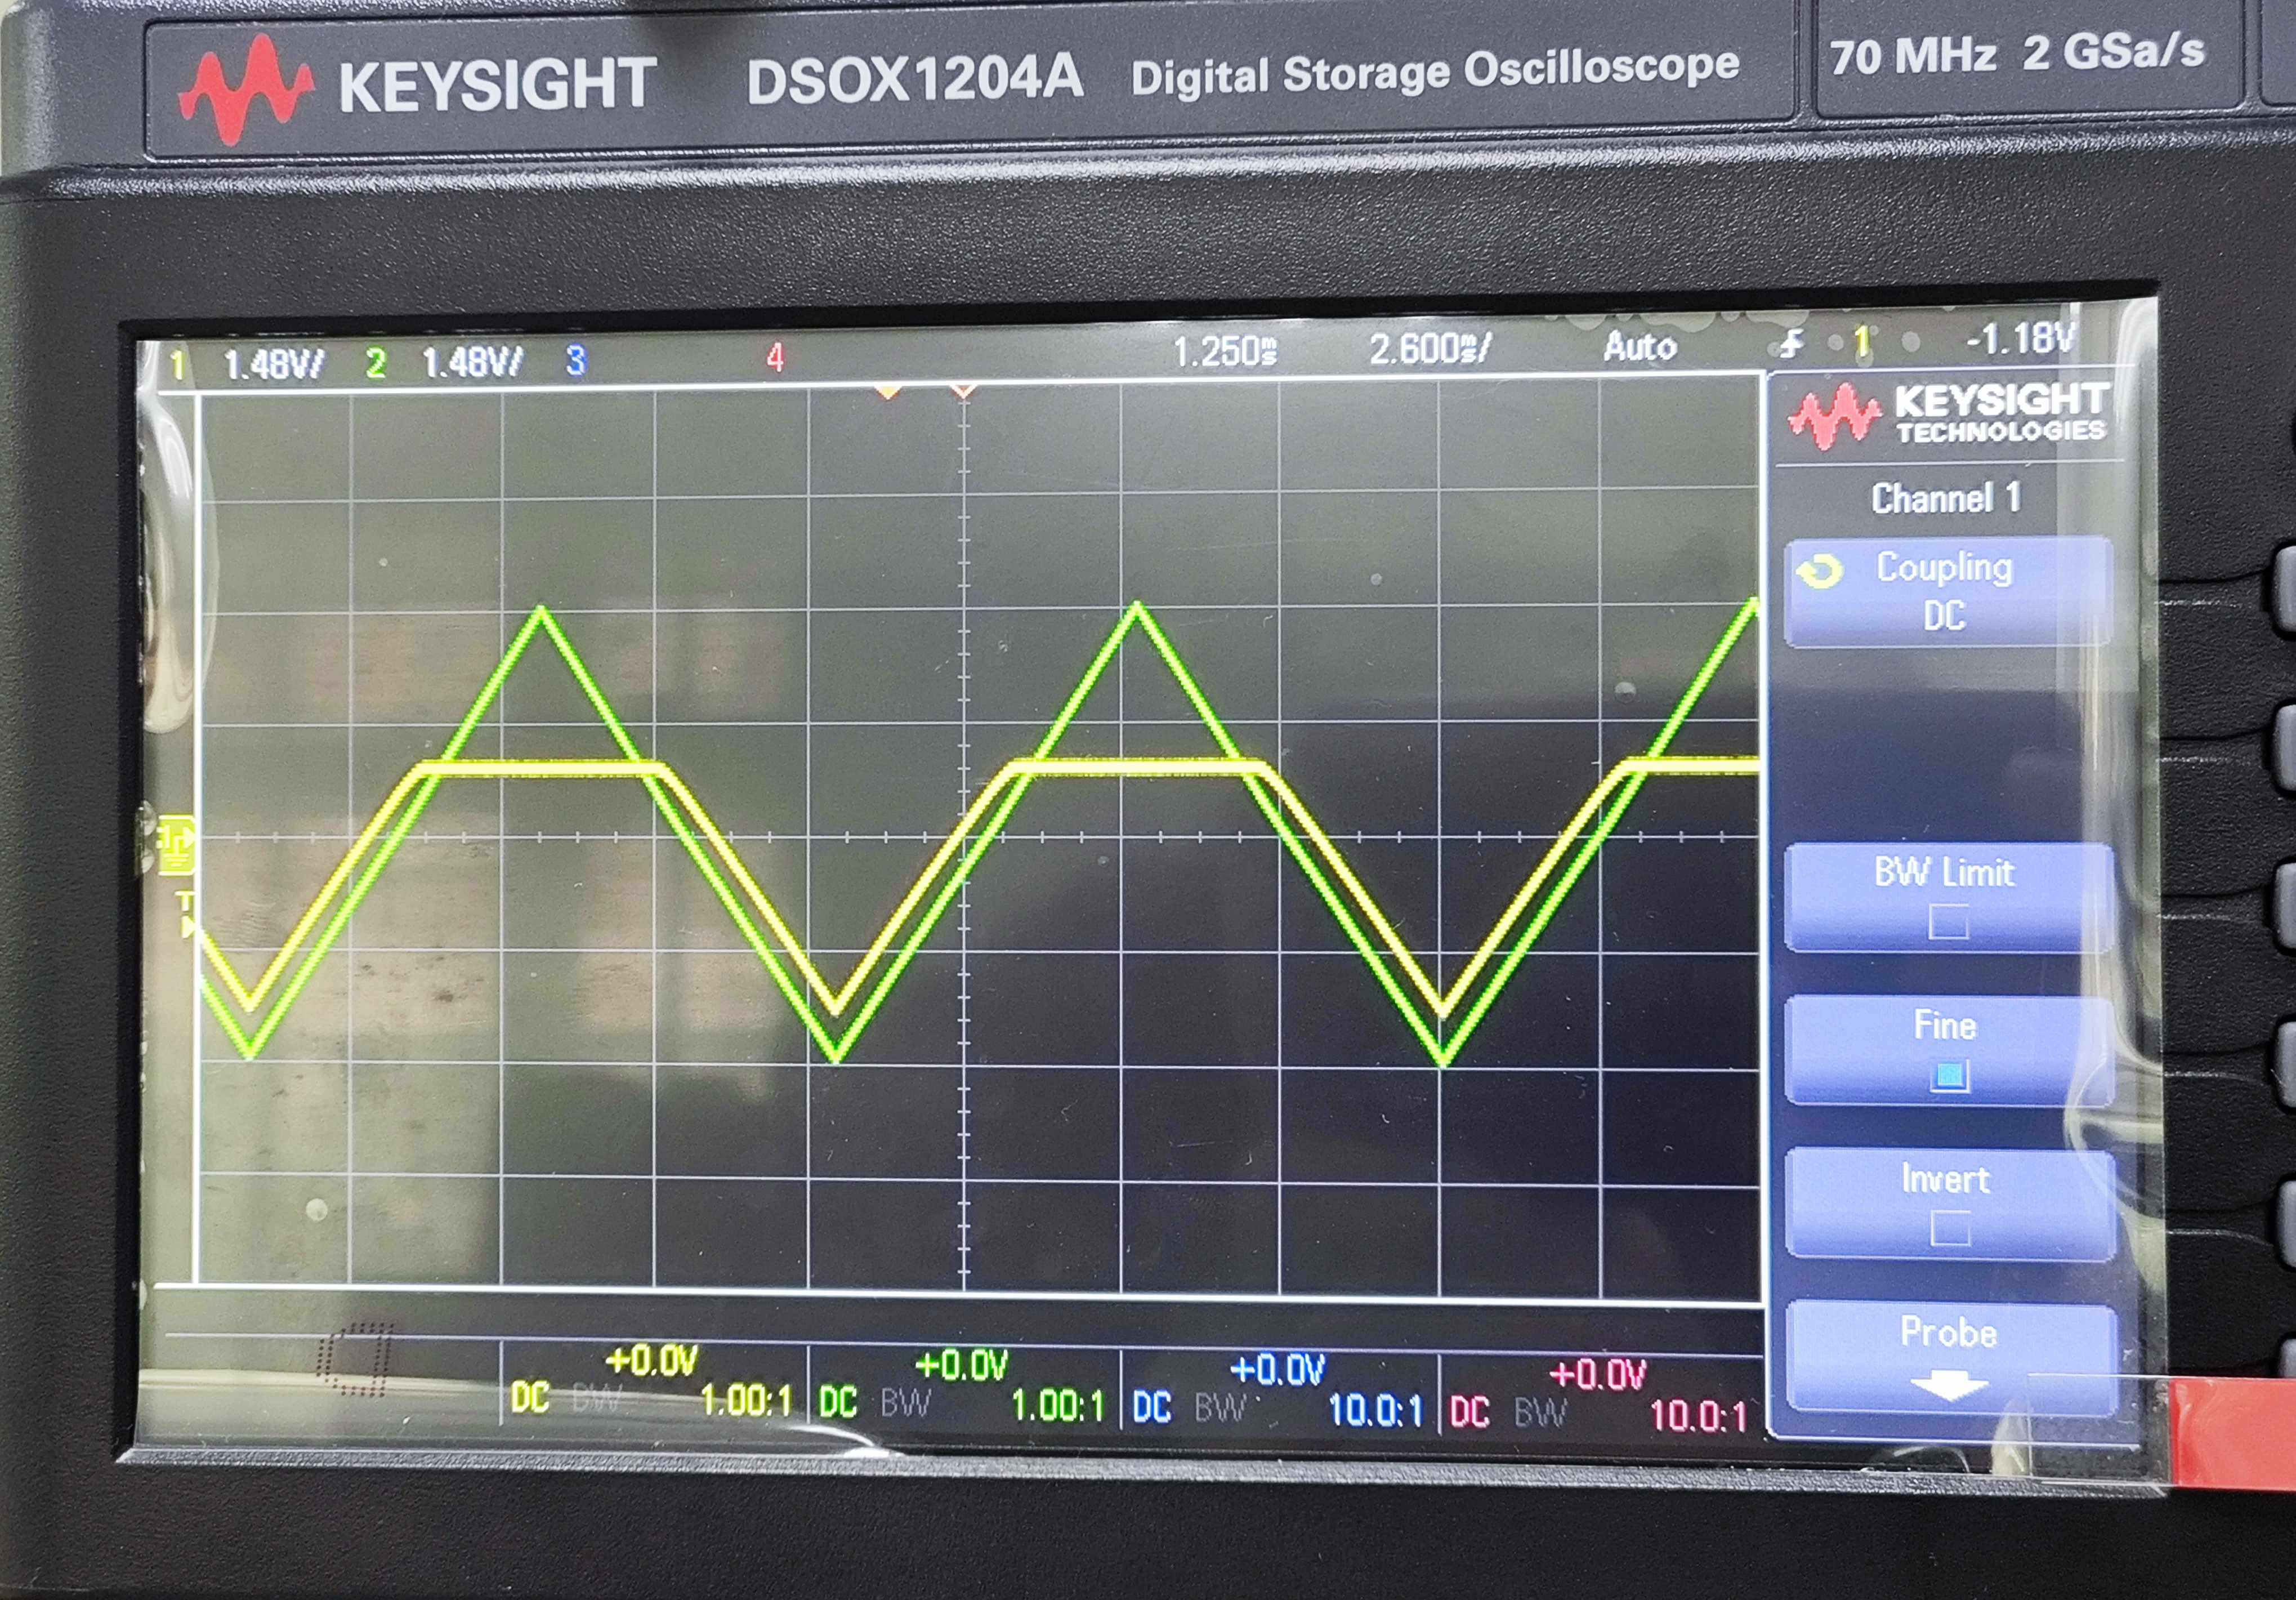
\includegraphics[width=0.65\linewidth]{Lab02/2.5_tri_clipper1.jpg}
                \caption{Triangular Signal}
                \label{2.5tri}
            \end{figure}
            \FloatBarrier
            From the Fig.\ref{2.5sin} and Fig.\ref{2.5tri}, we can tell that part of positive signal is clipped and less amplitude with minor latency, those are caused by the existence of the diode. When input signal is greater than $V_B - V_\gamma$, the diode will be off then cut the positive signal from $V_s$ so the signal maintained until it is lower than $V_B - V_\gamma$, the appearance of latency is caused by  input signal need to reach diode threshold voltage.
        \item For Fig.\ref{Lab2c},\par
            \begin{table}[h]
            \centering
            \begin{tabular}{|c|c|c|c|c|c|c|c|}
                \hline
                Vs   & 0     & 0.5   & 1     & 1.5   & 2     & 2.5   & 3     \\ \hline
                Vo   & 4.548 & 4.585 & 4.827 & 5.073 & 5.321 & 5.569 & 5.817 \\ \hline
                Theo & 4.449 & 4.449 & 4.449 & 4.449 & 4.449 & 4.449 & 4.449 \\ \hline
                Vs   & 3.5   & 4     & 4.5   & 5     & 5.5   & 6     & 6.5   \\ \hline
                Vo   & 6.066 & 6.312 & 6.561 & 6.805 & 7.05  & 7.294 & 7.534 \\ \hline
                Theo & 4.449 & 4.865 & 5.319 & 6.364 & 6.818 & 7.273 & 7.727 \\ \hline
                Vs   & 7     & 7.5   & 8     & 8.5   & 9     & 9.5   & 10    \\ \hline
                Vo   & 7.765 & 7.966 & 7.994 & 7.994 & 7.994 & 7.994 & 7.994 \\ \hline
                Theo & 7.137 & 8     & 8     & 8     & 8     & 8     & 8     \\ \hline
            \end{tabular}
            \end{table}
            \FloatBarrier
            \begin{figure}[h]
                \centering
                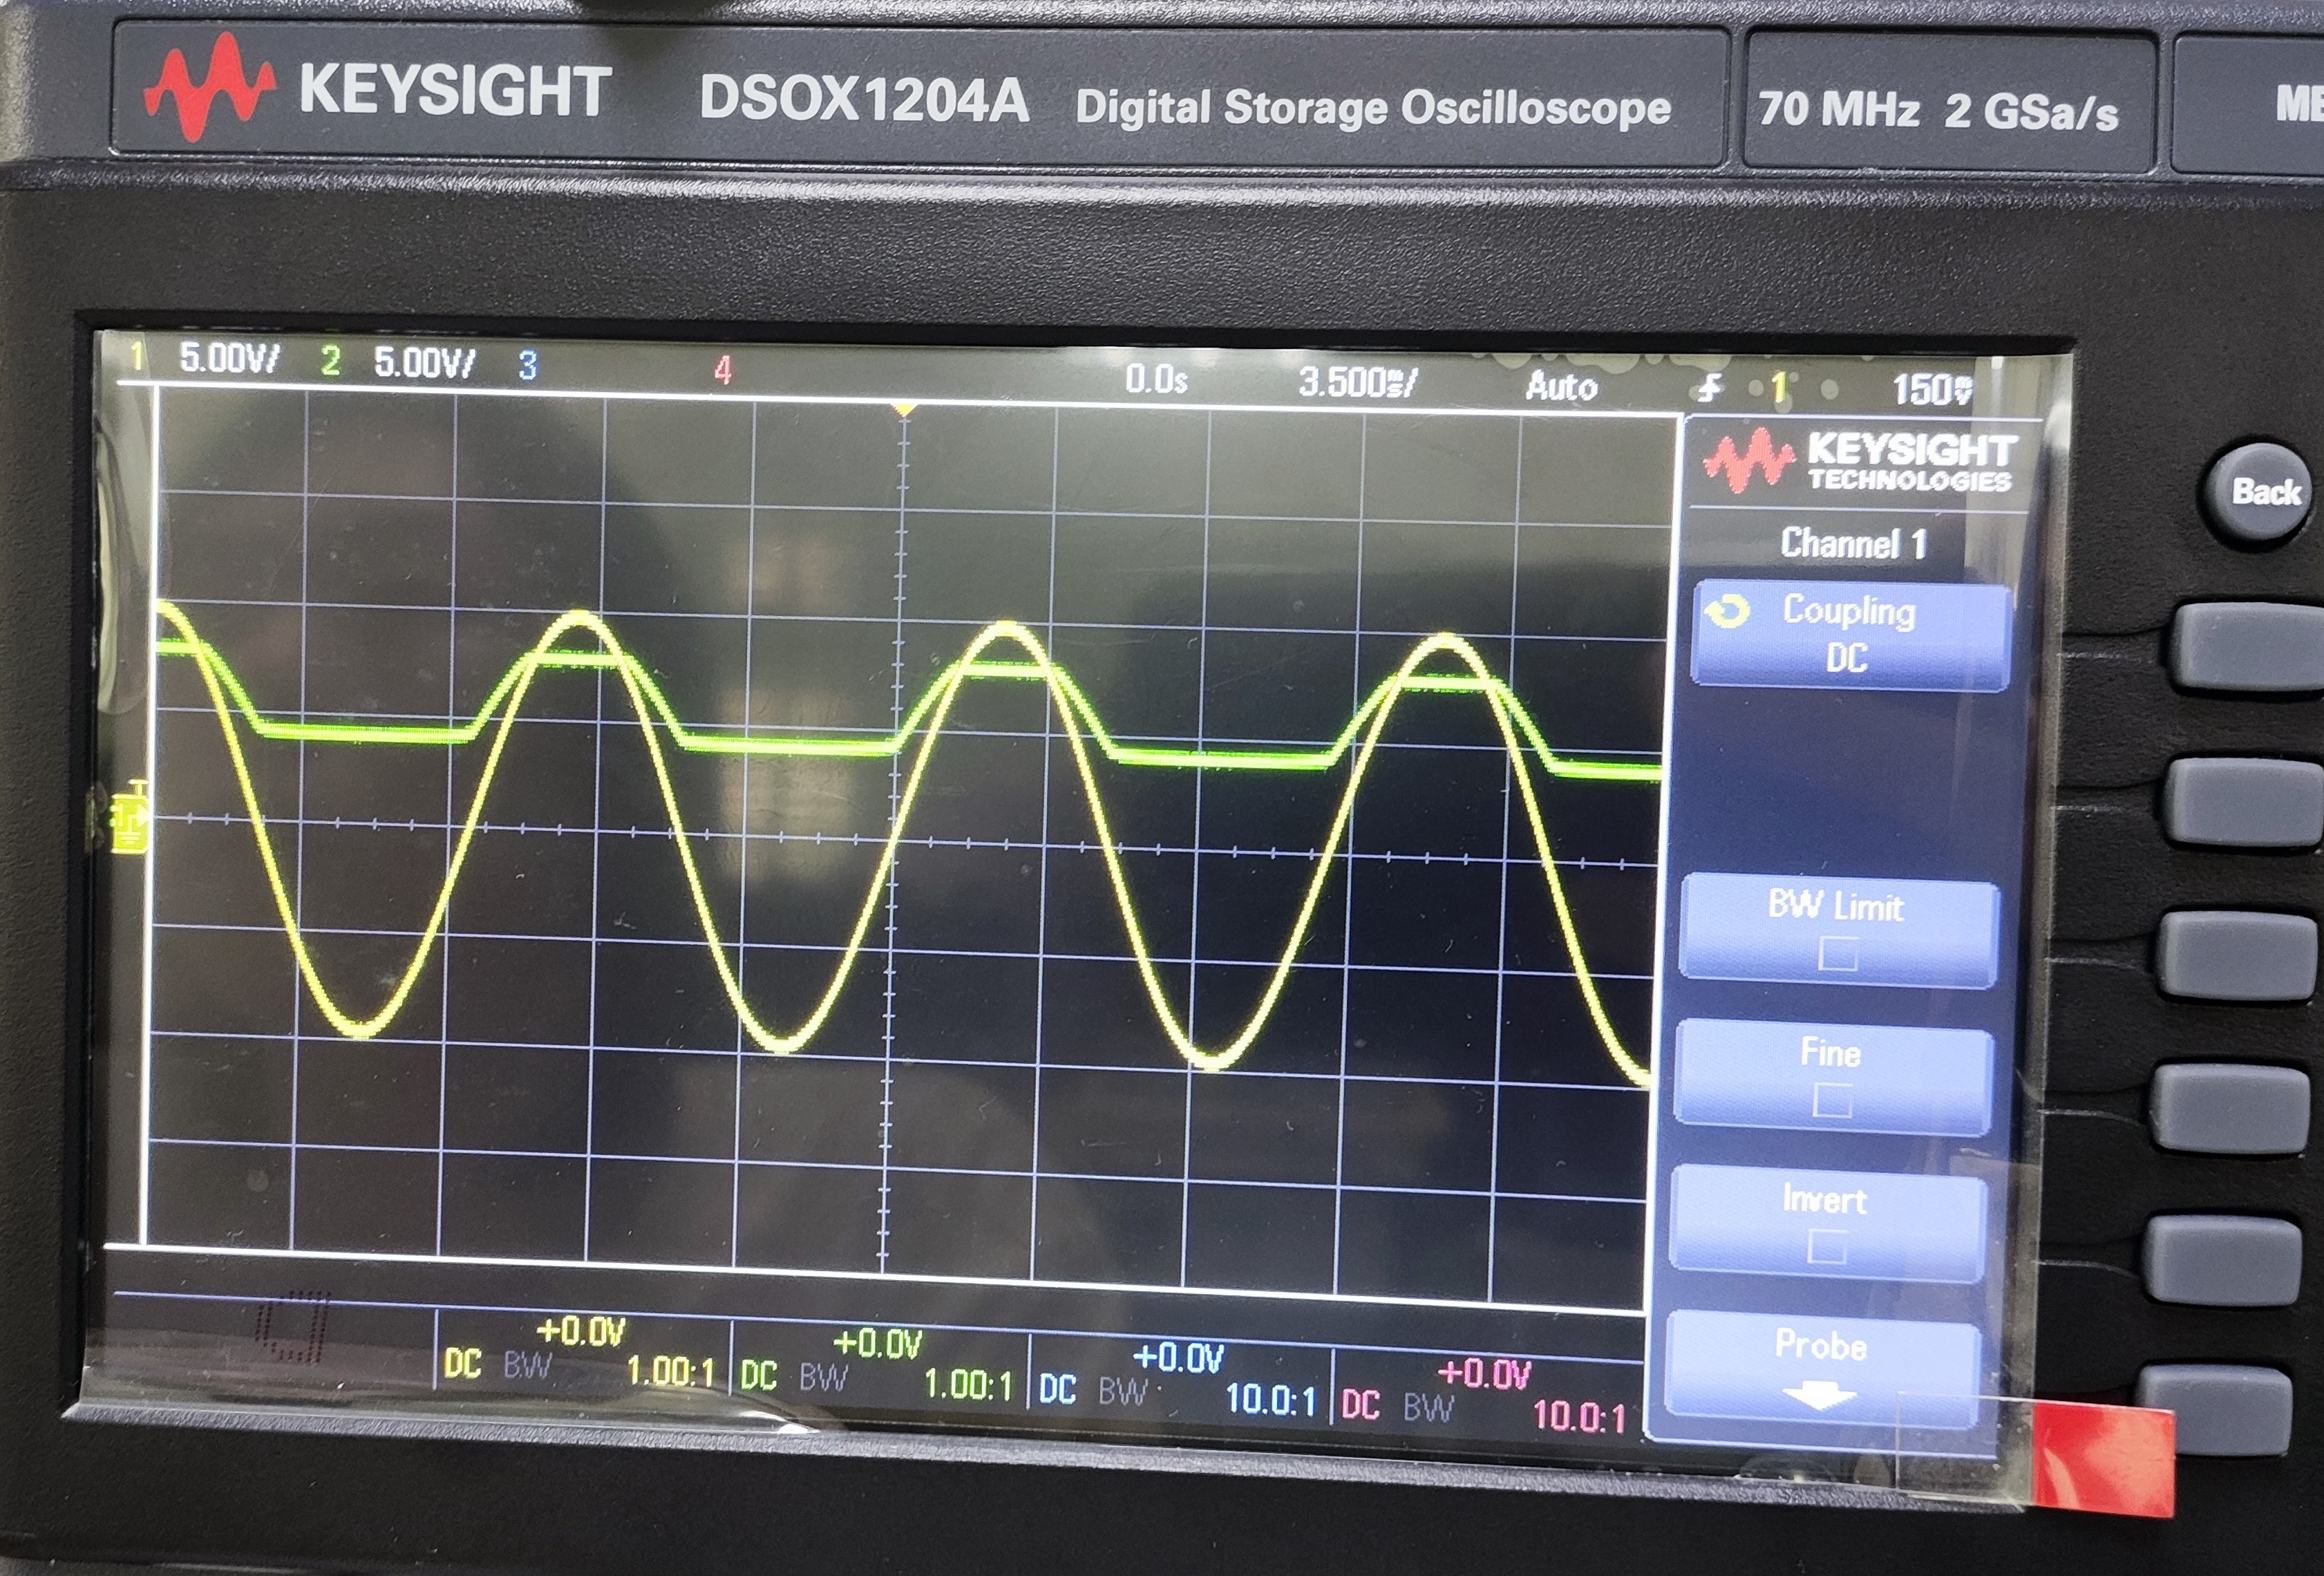
\includegraphics[width=0.65\linewidth]{Lab02/2.6_sin_clipper2.jpg}
                \caption{Sinusoidal Signal}
                \label{2.6sin}
            \end{figure}
            \FloatBarrier
            \begin{figure}[h]
                \centering
                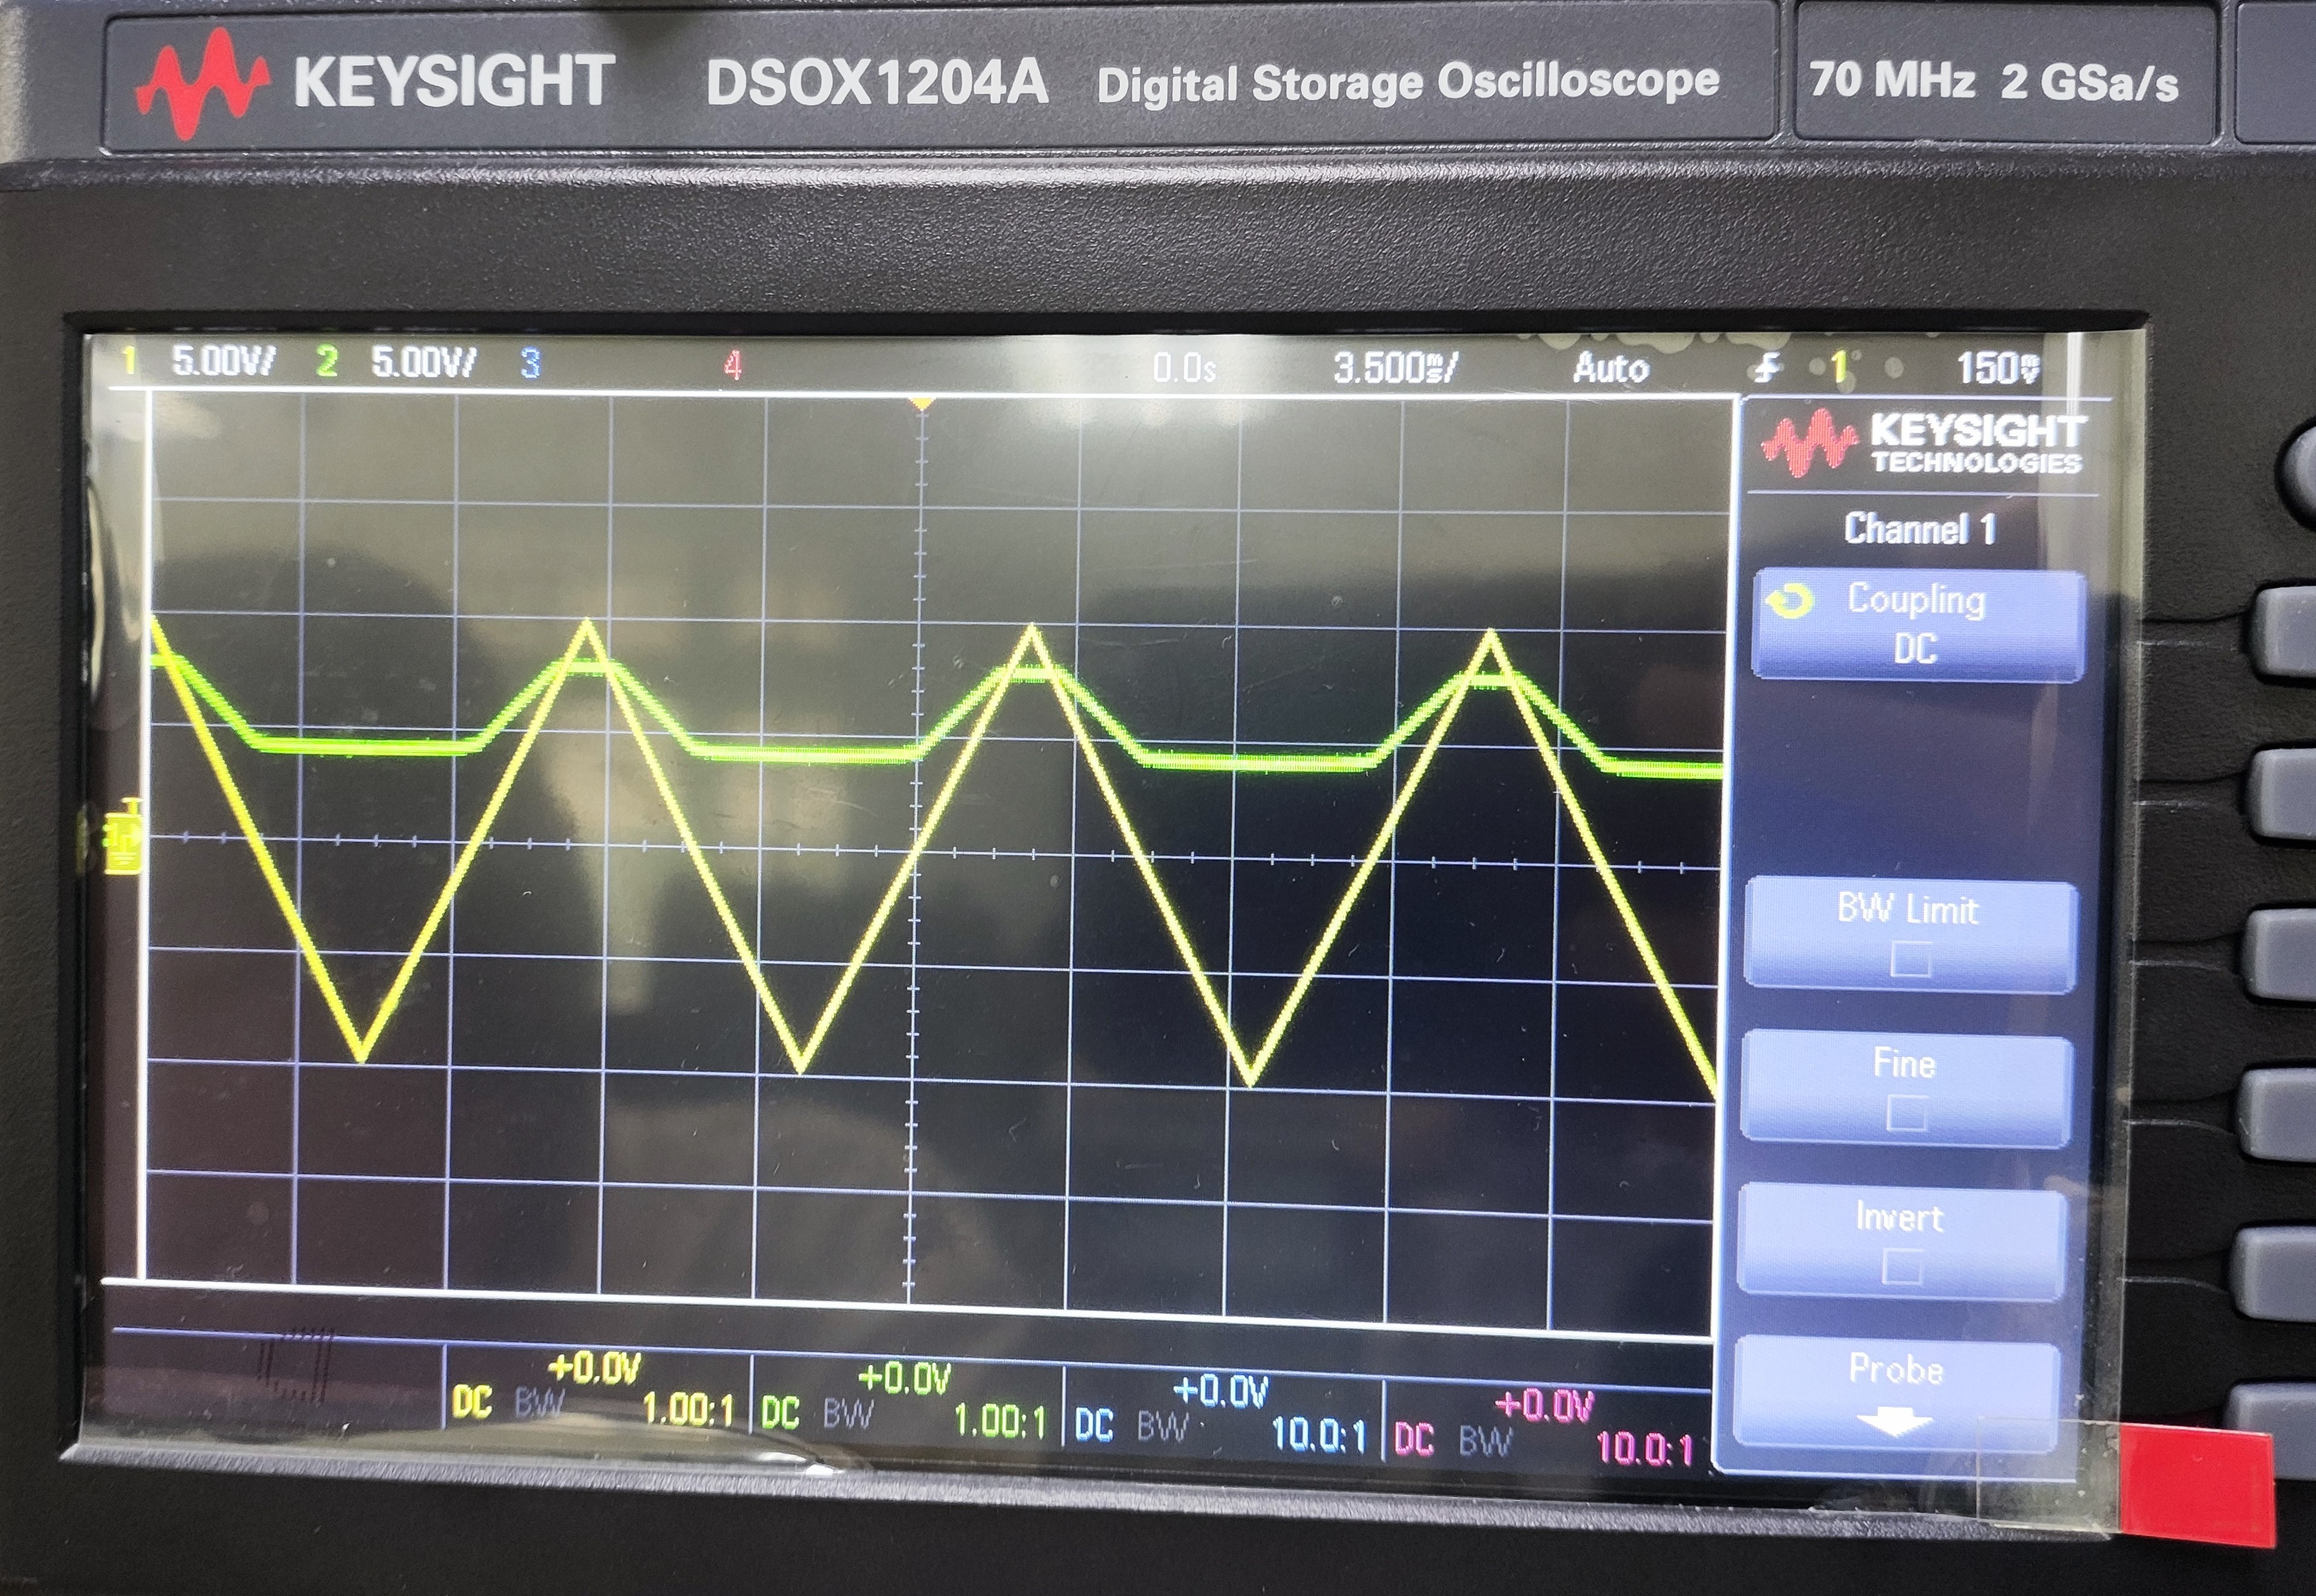
\includegraphics[width=0.65\linewidth]{Lab02/2.6_tri_clipper2.jpg}
                \caption{Triangular Signal}
                \label{2.6tri}
            \end{figure}
            \FloatBarrier
            This circuit is clipped twice, it is limited in the positive axis within the range of 4.449V to 8V. we still can see the latency of signal when it is rising and falling in both figures, it is because the input signal need to dissipate voltage on diode to reach its threshold voltage as well.

            \item For Fig.\ref{Lab2d},
            \begin{figure}[h]
                \centering
                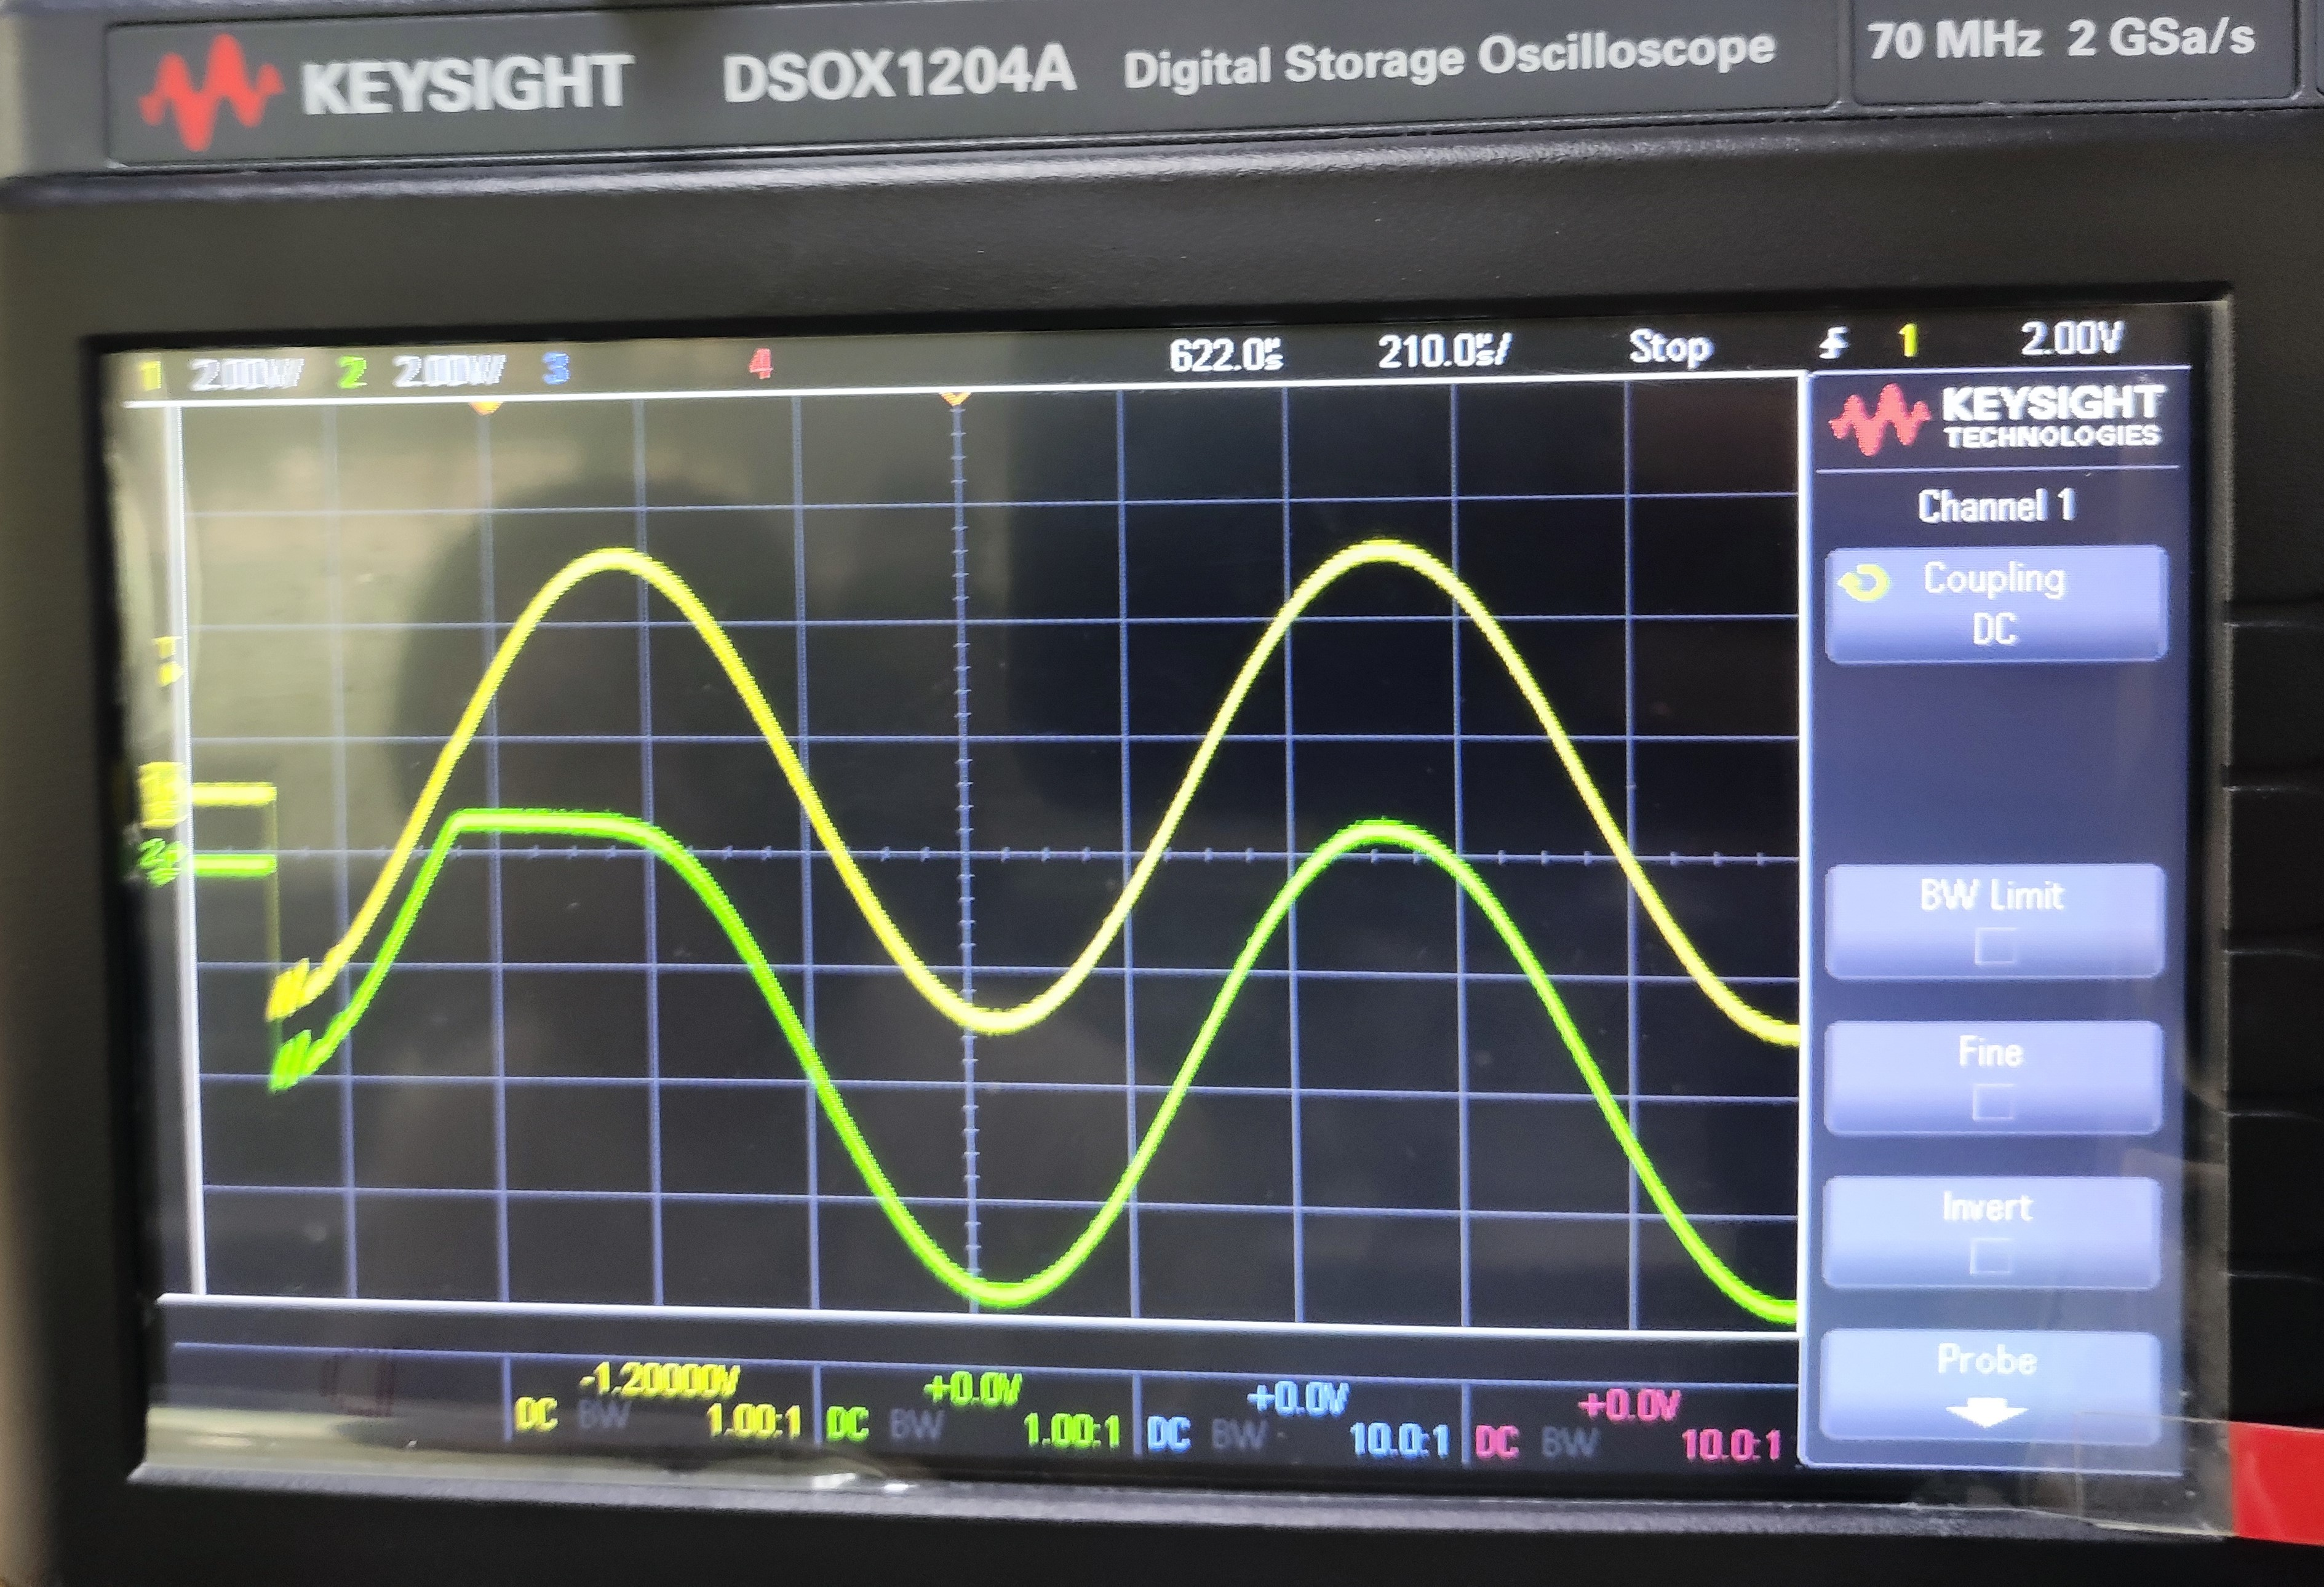
\includegraphics[width=0.65\linewidth]{Lab02/2.7_sin_clamper.jpg}
                \caption{Clamper Circuit Waveform}
                \label{2.7clamper}
            \end{figure}
            \FloatBarrier
            In Fig.\ref{2.7clamper}, Channel 1 (Yellow) is input and Channel 2 (Green) is output. It shows that the signal amplitude is shifted toward to negative axis. When the function generator provides positive signal, the diode conducts and the capacitor charges, when the function generator outputs negative signal, the diode is reverse-biased, the $V_o$ shifts downward, then the resulting waveform will be shifted toward negative axis.
    \end{itemize}
    
\section{Discussion}
    The measured value of circuit in Fig.\ref{Lab2c} is different with theoretical value, this may be caused by using wrong resistors when the experiment conducts.

\section{Conclusion}
    During this experiment, I learned more about the circuit contains diodes, and what the diode circuits can do. I understand the practical usage of diode circuit after conducting this experiment.